\hypertarget{index_Introduction}{}\section{Introduction}\label{index_Introduction}
Determining dead and noisy channels is based on the analysis of the channel A\-D\-C spectra recorded during a P\-M\-Noise\-Run. These spectra are provided by {\ttfamily ahc\-Bin\-Hst} from the {\ttfamily calice\-\_\-daq} package.

 
\begin{DoxyImage}
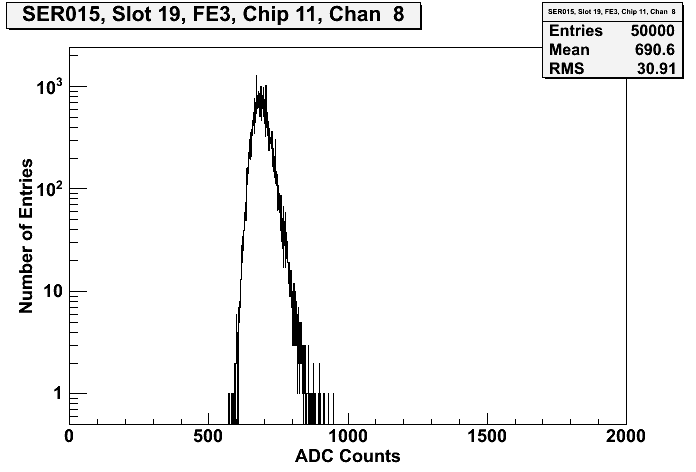
\includegraphics[width=0.7\textwidth]{normal_channel_spectrum.png}
\caption{Typical A\-D\-C spectrum of a channel in a noise run.}
\end{DoxyImage}


Only the mean of the distribution (the pedestal in case of a noise run) and the width (R\-M\-S) are used.\hypertarget{index_Definition}{}\section{Definition of dead and noisy}\label{index_Definition}
Currently dead and noisy are only defined from the R\-M\-S. \hypertarget{index_Noisy}{}\subsection{Noisy}\label{index_Noisy}
Looking at R\-M\-S sectrum of all channels one sees that most channels have an R\-M\-S around 40, but some channels (the noisy ones) have much larger R\-M\-S, causing a tail in the distribution.

 
\begin{DoxyImage}
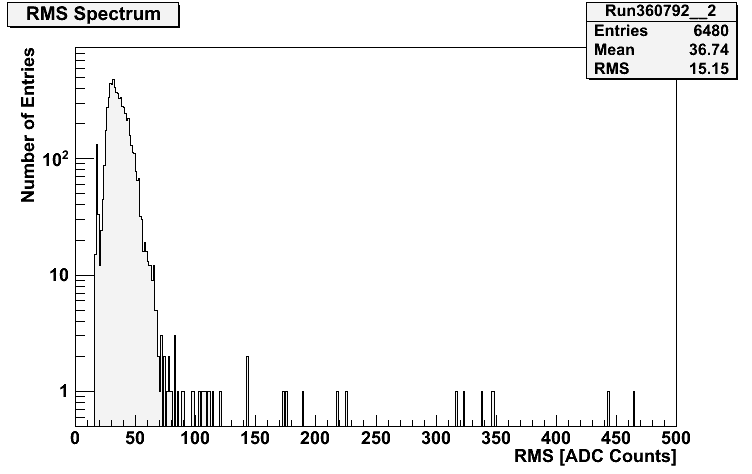
\includegraphics[width=0.7\textwidth]{rms_spectrum.png}
\caption{The R\-M\-S spectrum of all channels.}
\end{DoxyImage}


{\bfseries Definiton of noisy\-: R\-M\-S $>$ 140 }\hypertarget{index_Dead}{}\subsection{Dead}\label{index_Dead}
A comparisan with data and L\-E\-D\-V\-Calib runs has shown that the peak at the lover end of the distribution contains basically only dead channels (see section \char`\"{}\-Comparing two runs\char`\"{}).

 
\begin{DoxyImage}
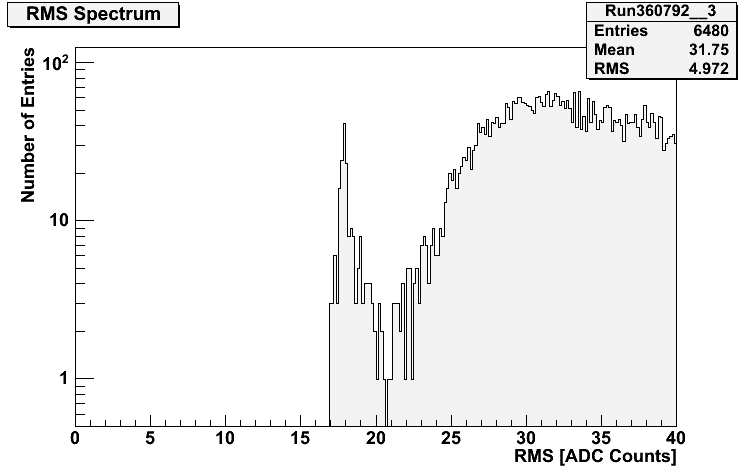
\includegraphics[width=0.7\textwidth]{rms_spectrum_zoom.png}
\caption{The R\-M\-S spectrum of all channels.}
\end{DoxyImage}


{\bfseries Definiton of dead\-: R\-M\-S $<$ 20.\-5 }\hypertarget{index_SWOverview}{}\section{Software overview}\label{index_SWOverview}
The software basically consists of two parts \begin{DoxyItemize}
\item The root library {\ttfamily lib\-Dead\-And\-Noisy\-Tools} which conveniently allows to access the R\-M\-S and pedestal values of one or several runs \item The {\ttfamily create\-Bad\-Channels\-List} executable which creates the list of bad channels to be written to the database.\end{DoxyItemize}
\hypertarget{index_pages}{}\subsection{Detailed descritons}\label{index_pages}
\begin{DoxyItemize}
\item \hyperlink{download_install}{Download and Installation} \item The \hyperlink{create_bad_channels_list_exe}{create\-Bad\-Channels\-List} executable \item The \hyperlink{root_lib}{lib\-Dead\-And\-Noisy\-Tools} root library \item \hyperlink{_examples}{Examples}\end{DoxyItemize}
\hypertarget{index_Outlook}{}\section{Outlook}\label{index_Outlook}
\begin{DoxyRefDesc}{Todo}
\item[\hyperlink{todo__todo000007}{Todo}]Implement convenience draw functions which create the default plots with well formated axis labels etc. 

Transfer missing functionality from C scripts. 

Maybe implement G\-U\-I?\end{DoxyRefDesc}
